\documentclass[a4paper,ngerman]{article}

%%%%%%%%%%%%%%%%%%%%%%%%%%%%%%%%%%%%%%%%%%%%%%%%%%%%%%%%%%%%%%%%%%%%%%%%%%%%%%%%%%%%%%%%%%%%%%%%%%%
%% allgemeine LaTeX Pakete laden
%%%%%%%%%%%%%%%%%%%%%%%%%%%%%%%%%%%%%%%%%%%%%%%%%%%%%%%%%%%%%%%%%%%%%%%%%%%%%%%%%%%%%%%%%%%%%%%%%%%

% Mathematik
\usepackage{amsmath}  % American Math Society Packete: general
\usepackage{amsfonts} % American Math Society Packete: more fonts
\usepackage{amssymb}  % American Math Society Packete: more symbols
\usepackage{stmaryrd} % St Mary Road symbols for theoretical computer science
\usepackage[framed,hyperref,amsmath,thmmarks]{ntheorem} % en­hance­ments for the­o­rem-like en­vi­ron­ments

% Umlaute tippen
\usepackage[utf8]{inputenc}

% Wörterbuch für korrekte Silbentrennung, Titel von Abschnitten (Abbildung, Zusammenfassung, Literaturverzeichnis)
\usepackage{babel}

% Blockweises auskommentieren mit \begin{comment}\end{comment}
\usepackage{verbatim}

% Grafiken 
\usepackage{graphics,graphicx} % Bilder
\usepackage{color,xcolor} % Farbnamen
\graphicspath{{figures/}} % Es gibt ein Unterverzeichnis, wo alle Bilder liegen. Durch diesen Befehl muss man nicht jedes mal den Dateipfad angeben

%Listen
\usepackage{enumerate}
\usepackage{enumitem}

%Tabellen
\usepackage{tabularx}
\usepackage{booktabs}% Statt \hline kann \toprule, \midrule und \bottomrule verwendet werden.
\usepackage{longtable}
\usepackage{tabularray}
\usepackage{multicol} % to use columns with multiple rows
%\usepackage{multirow} % provides a construction for table cells that span more than one row

% Algorithmen
\usepackage{algorithm}
\usepackage{algorithmic}
% Algorithmen auf Deutsch %
\renewcommand{\algorithmicrequire}{\textit{Eingabe:}}
\renewcommand{\algorithmicensure}{\textit{Ausgabe:}}
\floatname{algorithm}{Algorithmus}

%Referenzen
\usepackage[unicode,pdfmenubar,linktoc=all,hidelinks,bookmarks]{hyperref} % ermöglicht PDF-Verklinkungen
\usepackage{url} % al­lows line­breaks at cer­tain char­ac­ters in urls/ e-mail adresses/ paths
%\usepackage{thmtools}%für nameref von Theoremen, aber dann sind Nummern bei Lemma/Korollar weg
\usepackage[nameinlink, compress, sort]{cleveref}% Kommando \Cref{label} schreit automatisch Abbildung/Abschnitt/Tabelle vor die Referenz
\usepackage{nameref}

%%%%%%%%%%%%%%%%%%%%%%%%%%%%%%%%%%%%%%%%%%%%%%%%%%%%%%%%%%%%%%%%%%%%%%%%%%%%%%%%%%%%%%%%%%%%%%%%%%%
%% Tikz Grafiken
%%%%%%%%%%%%%%%%%%%%%%%%%%%%%%%%%%%%%%%%%%%%%%%%%%%%%%%%%%%%%%%%%%%%%%%%%%%%%%%%%%%%%%%%%%%%%%%%%%%
\usepackage{tikz}
% Zusätzliche Tikz-Module einbinden
\usetikzlibrary{automata} 
\usetikzlibrary{arrows}
\usetikzlibrary{calc}
\usetikzlibrary{positioning}

% Tikz-Stil für Automaten
\tikzset{
	myautomat/.style = {
		>=stealth, shorten >= 1pt,auto,node distance=2cm,
	}
}
\tikzstyle{initial}+=[initial text=]

%Definiere hier eigene Tikz-Styles, damit alle Grafiken (z.B. alle Graphen) in einem einheitlichen Stil sind

%%%%%%%%%%%%%%%%%%%%%%%%%%%%%%%%%%%%%%%%%%%%%%%%%%%%%%%%%%%%%%%%%%%%%%%%%%%%%%%%%%%%%%%%%%%%%%%%%%%
%% Literatur
%%%%%%%%%%%%%%%%%%%%%%%%%%%%%%%%%%%%%%%%%%%%%%%%%%%%%%%%%%%%%%%%%%%%%%%%%%%%%%%%%%%%%%%%%%%%%%%%%%%
\usepackage[style=alphabetic,backend=biber]{biblatex}
\bibliography{literatur}

%%%%%%%%%%%%%%%%%%%%%%%%%%%%%%%%%%%%%%%%%%%%%%%%%%%%%%%%%%%%%%%%%%%%%%%%%%%%%%%%%%%%%%%%%%%%%%%%%%%
%% Theoreme 
%%%%%%%%%%%%%%%%%%%%%%%%%%%%%%%%%%%%%%%%%%%%%%%%%%%%%%%%%%%%%%%%%%%%%%%%%%%%%%%%%%%%%%%%%%%%%%%%%%%

%Definiere Umgebungen für Aussagen
\newtheorem{theorem}{Theorem}% (wichtiger Satz) Höhepunkt in der Entwicklung einer Theorie
\newtheorem{corollary}[theorem]{Korollar}% (Folgerung) einfach/ trivial aus vorhergehenden Sätzen zu folgern 
\newtheorem{lemma}[theorem]{Lemma}% (Hilfssatz) rein technische Aussage, als Schlüsselgedanke für anderen Beweis
\newtheorem{proposition}[theorem]{Proposition}%  Mittelding aus Hilfssatz und Theorem
\newtheorem{observation}[theorem]{Beobachtung}

\newtheorem{example}[theorem]{Beispiel}
\newtheorem{definition}[theorem]{Definition}
\newtheorem{problem}[theorem]{Problem}
\newtheorem{remark}[theorem]{Bemerkung}

% Beweis-Umgebung
\theorembodyfont{\upshape}
\theoremstyle{nonumberplain}
\theoremheaderfont{\itshape}
\theoremsymbol{\ensuremath{\Box}}%QED Symbol am Beweisende
\newtheorem{proof}{Beweis}

% Zeilennummern
\usepackage{lineno}

%%%%%%%%%%%    Meta Informationen   %%%%%%%%%%%%%%
\title{Titel des Themas\\
{\normalsize Proseminar:  Titel des Proseminar}
}
\author{Dein Name}
\date{\today}

\begin{document}

\maketitle

%%%%%%%%%%%    Ausarbeitung   %%%%%%%%%%%%%%
\linenumbers % Ab hier werden die Zeilen gezählt
	
\begin{abstract}
	Kurze Zusammenfassung, worum es in dieser Ausarbeitung geht.
\end{abstract}

\section{Einleitung}
\label{sec:intro}

Führe hier in das Thema ein: Worum geht es? Warum ist dies interessant? Welche Ergebnisse werden vorgestellt? Aufbau der Arbeit?

\section{Hauptteil}


Gebe hier eine abgeschlossene Darstellung des Inhaltes. Schreibe diese so, dass sie für Deine Kommilitonen verständlich ist. Verwende dabei zur Anschauung des Inhaltes auch Beispiele und Abbildungen.

\subsection{Hinweise}

Der Hauptteil soll natürlich nicht den Titel \glqq Hauptteil\grqq\ sondern einen passenden Titel haben, und zudem in sinnvolle Abschnitte und Unterabschnitte mit passenden Überschriften gegliedert sein.

\subsection{Zitate und Referenzen}
Denke daran, alle Aussagen durch Quellen zu belegen. Beispielsweise die Aussage, dass Turing die Unentscheidbarkeit des Halteproblems gezeigt hat \cite{Turing1937}.

Um innerhalb der Ausarbeitung zu referenzieren, können Bereiche mit einem \texttt{label} versehen werden. Durch das Paket \texttt{cleverref} wird beim Referenzieren automatisch [Abbildung/ Abschnitt/ Tabelle/ etc.] ergänzt. Beispiele in diesem Dokument sind \Cref{sec:intro,fig:automat,alg:BFS,theo:aussage}.

\begin{figure}
	\centering
	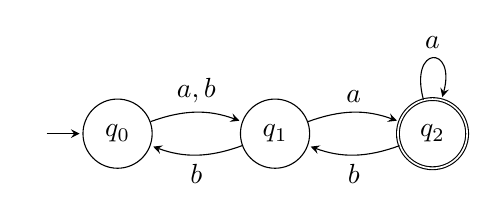
\begin{tikzpicture}[myautomat]
		\node[state, initial] (0) {$q_0$};
		\node[state] (1) [right of=0] {$q_1$};
		\node[state, double] (2) [right of=1] {$q_2$};
		
		\draw[->] (0) edge[bend left=20] node[auto] {$a,b$} (1);
		\draw[->] (1) edge[bend left=20] node[auto] {$a$} (2)
		edge[bend left=20] node[auto] {$b$} (0);
		\draw[->] (2) edge[loop above] node[auto] {$a$} () 
		edge[bend left=20] node[auto] {$b$} (1);
	\end{tikzpicture}
	\caption{Ein Automat, der mit Tikz erzeugt wurde}
	\label{fig:automat}
\end{figure}

\begin{figure}
	\centering
	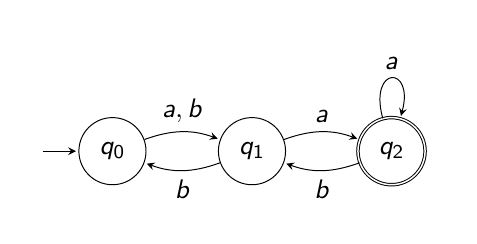
\includegraphics[width=8cm]{automat.jpg} 
	\caption{Eine Automat, der als jpg-Bild eingebunden wurde (Achtung: Auflösung!)}
\end{figure}

\begin{theorem}[Besondere Formel]\label{theo:aussage}
	Hier ist eine Aussage.
\end{theorem}
\begin{proof}
	Hier folgt der Beweis.
\end{proof}

\begin{algorithm}
	\caption{Breitensuche (BFS)}
	\label{alg:BFS}
	\begin{algorithmic} []
		\REQUIRE Graph $G$, Startknoten $s$, leere Warteschlange $Q$
		\ENSURE BFS
		
		\STATE	$Q$.enqueue($s$)			
		\STATE mark $s$ as visited
		\WHILE{$Q$ is not empty}
		\STATE	$v$ = $Q$.dequeue( )			
		\FORALL{neighbors $w$ of $v$}
		\IF{$w$ is not visited}
		\STATE	$Q$.enqueue($w$)
		\STATE	mark $w$ as visited
		\ENDIF
		\ENDFOR
		\ENDWHILE
	\end{algorithmic}
\end{algorithm}


\section{Zusammenfassung und Ausblick}

Fasse hier die vorgestellten Ergebnisse zusammen, diskutiere diese und gebe einen Ausblick auf offene Fragen. 

%%%%%%%%%%%    Der folgende Teil zählt nicht zu Zeilenbeschränkung der Vorgabe   %%%%%%%%%%%%%%
\nolinenumbers

%%%%%%%%%%%    Literaturverzeichnis   %%%%%%%%%%%%%%
 \printbibliography 
 
 %%%%%%%%%%%    Anhang   %%%%%%%%%%%%%%
 \appendix
 
 \section{Eigenständigkeitserklärung und verwendete Hilfsmittel}
Ich versichere an Eides statt, dass ich die vorliegende Arbeit in allen Teilen selbstständig und ohne unzulässige Hilfe Dritter absolviert sowie keine anderen als die genannten und explizit zugelassenen Hilfsmittel verwendet und mich im Allgemeinen prüfungskonform verhalten habe. Ich erkläre zudem, dass ich beim Einsatz von IT-/KI-gestützten Schreibwerkzeugen diese Werkzeuge in der Übersicht verwendeter Hilfsmittel mit ihrem Produktnamen, meiner Bezugsquelle und … vollständig aufgeführt und/oder die betreffenden Textstellen in der Arbeit als mit KI generierter Unterstützung verfasst gekennzeichnet habe. Mir ist bewusst, dass Täuschungen bzw. Täuschungsversuche nach der für mich geltenden Prüfungsordnung geahndet werden.\\


Folgende Hilfsmittel habe ich für die Bearbeitung genutzt
 
\end{document}